Zur konkreten Realisierung wurde das System in 4 Teilsysteme unterteilt, welche separat betrachtet werden können. In jedem Gebiet wird auf die Anforderungen sowie verschieden mögliche Varianten eingegangen. Je nach Realisierbarkeit wird eine Variante gewählt, dimensioniert und die entsprechenden Komponenten ausgewählt.

\section{Vorversuche}


Da das Fließverhalten der Kunstoffe nur schwer abschätzbar ist, wird zur Erprobung ein vereinfachter Aufbau verwendet. In das Heizrohr ist ein Stahlrohr  eingeführt, welches das Original Keramik Innenrohr vor Verunreinigungen schützt. Die Probe wird Vertikal in das Rohr gehängt und Erwärmt, zu sehen in Abbildung \ref{fig:testaufbau}. Der Versuch soll Aufschluss über die nötige Abzugsgeschwindigkeit, Materialfördergeschwindigkeit und Form der Faser geben.


\begin{figure}[!h]
\centering
\begin{minipage}{.5\textwidth}
  \centering
  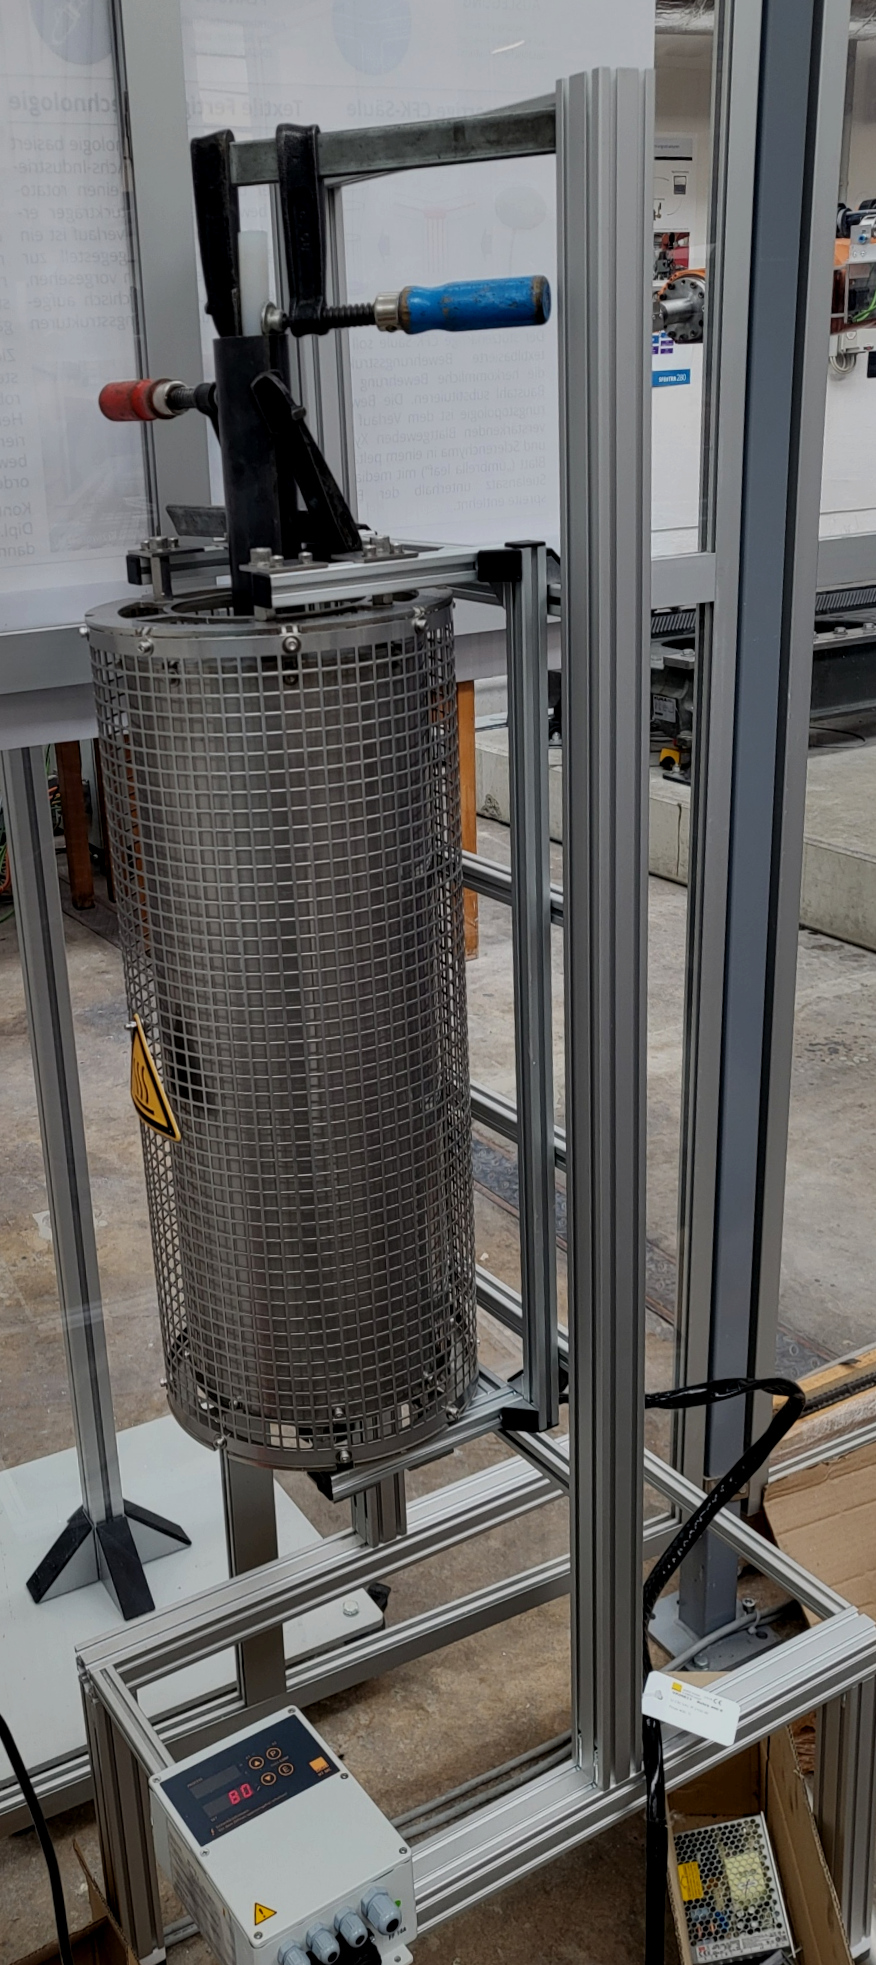
\includegraphics[width=.4\linewidth]{Abbildungen/Versuche/testaufbau_0010.jpg}
  \captionof{figure}{Testaufbau}
  \label{fig:testaufbau}
\end{minipage}%
\begin{minipage}{.5\textwidth}
  \centering
  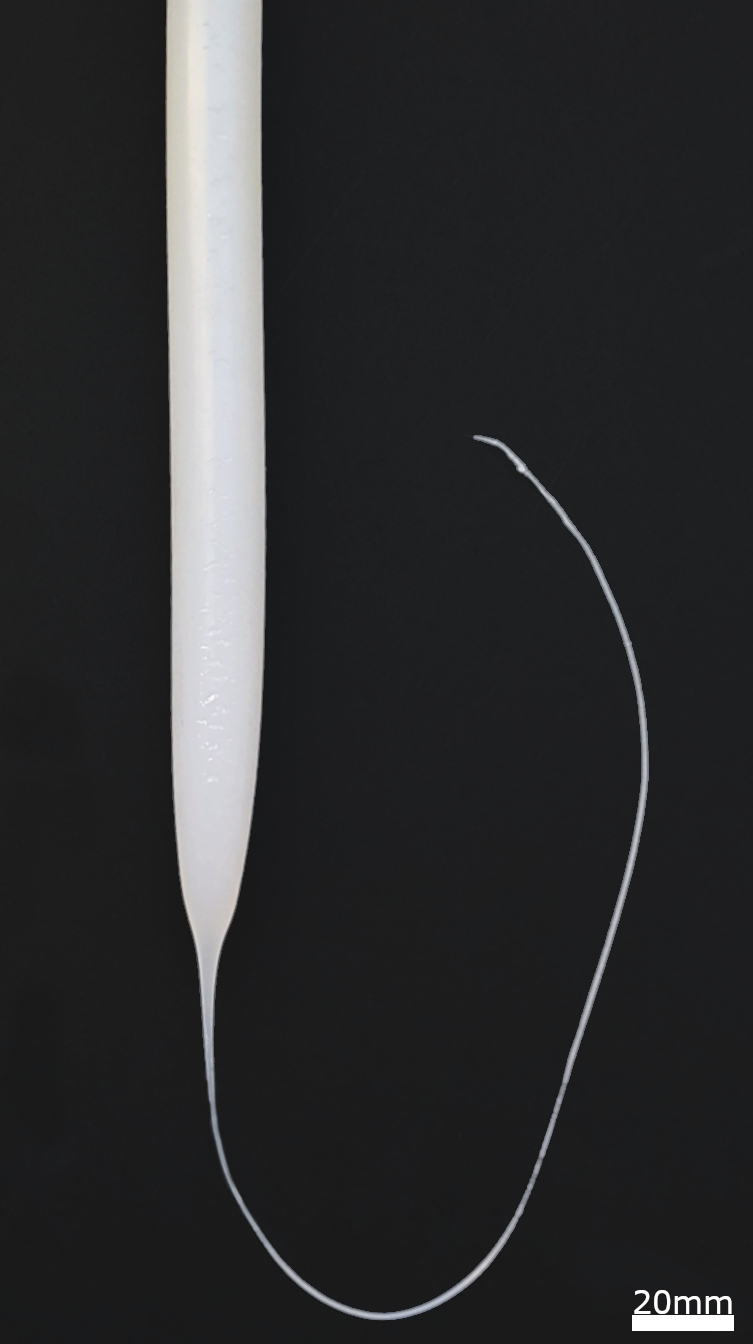
\includegraphics[width=.5\linewidth]{Abbildungen/Versuche/probe1_w.jpg}
  \captionof{figure}{\acs{evac}}
  \label{fig:probe1}
\end{minipage}
\end{figure}
 Die Erste Probe aus Abbildung \ref{fig:probe1} hat bei circa 205°C zu fließen begonnen. Dieser Versuch sollte nur veranschaulichen ob das gewählte Prinzip Funktionsfähig ist. Da sowohl die Faserdicke als auch die Fließform den erwartungen entsprechen, werden im nächsten Schritt andere Materialien verwendet. Um das Fließverhalten besser einschätzten zu können sind die folgenden Probenkörper mehrfarbig ausgeführt. Dadurch lässt sich beeurteilen wie die Faser aufgebaut ist. \newpage

 \begin{figure}[!h]
     \centering
     \begin{subfigure}[]{.29\textwidth}
         \centering
         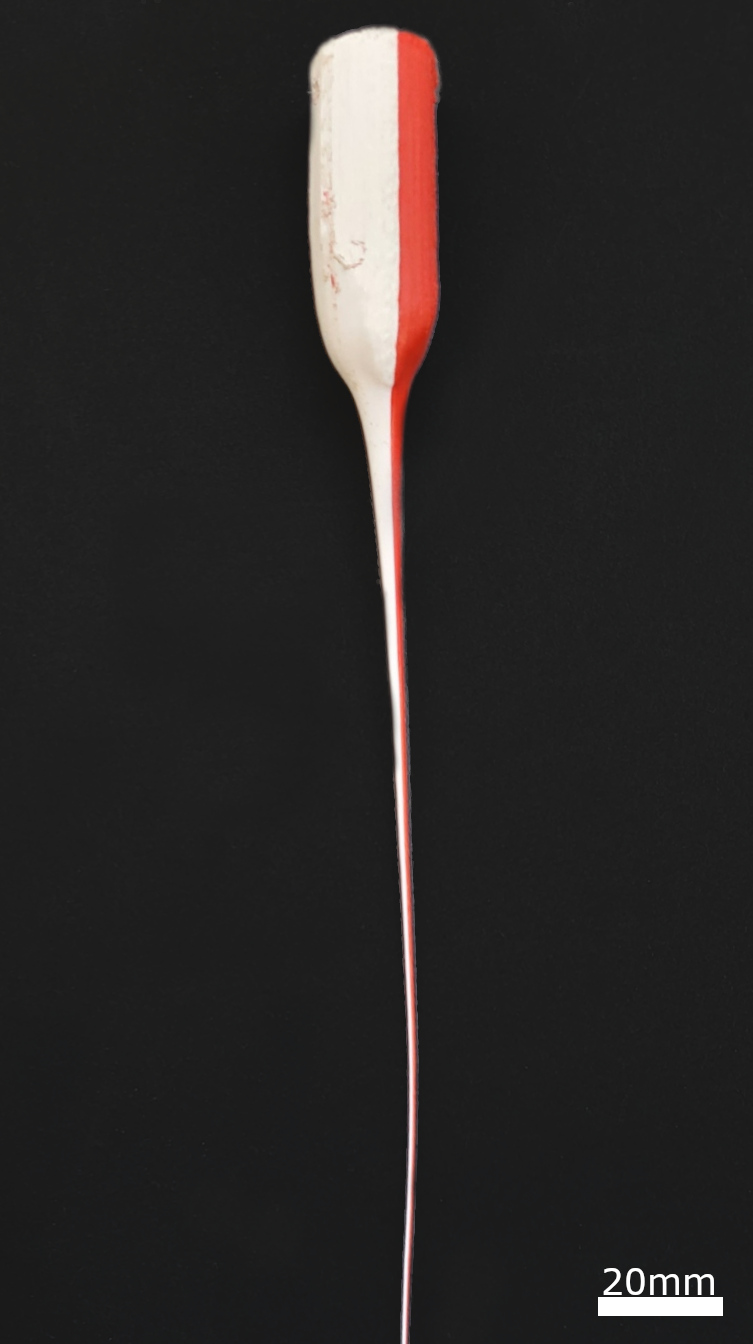
\includegraphics[width=\textwidth]{Abbildungen/Versuche/probe3_w.jpg}
         \caption{\acs{pla}/ \acs{pla}} 
         \label{fig:probe2}
     \end{subfigure}
     \hspace{5mm}
     \begin{subfigure}[]{.29\textwidth}
         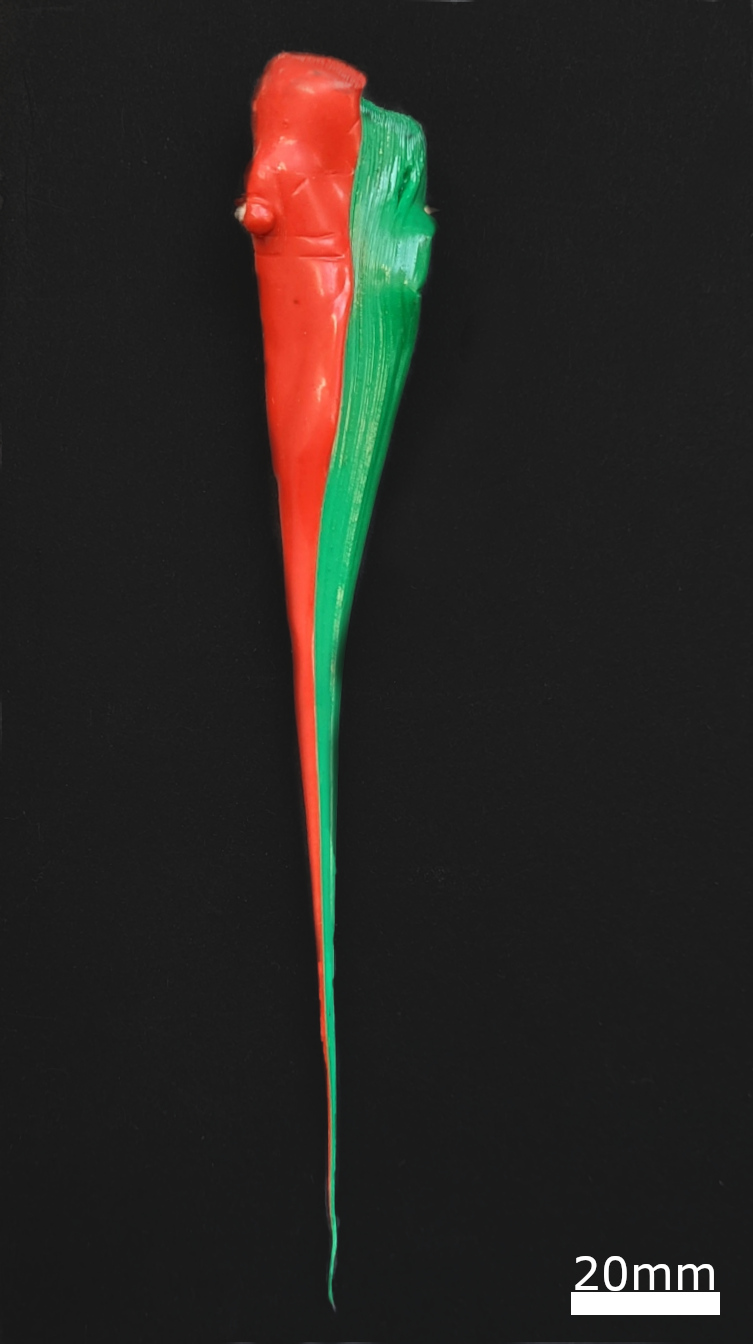
\includegraphics[width=\textwidth]{Abbildungen/Versuche/probe2_w.jpg}
         \caption{\acs{pla}/\acs{abs}}
         \label{fig:probe3}
     \end{subfigure}
     \hspace{5mm}
     \begin{subfigure}[]{.29\textwidth}
        \centering
        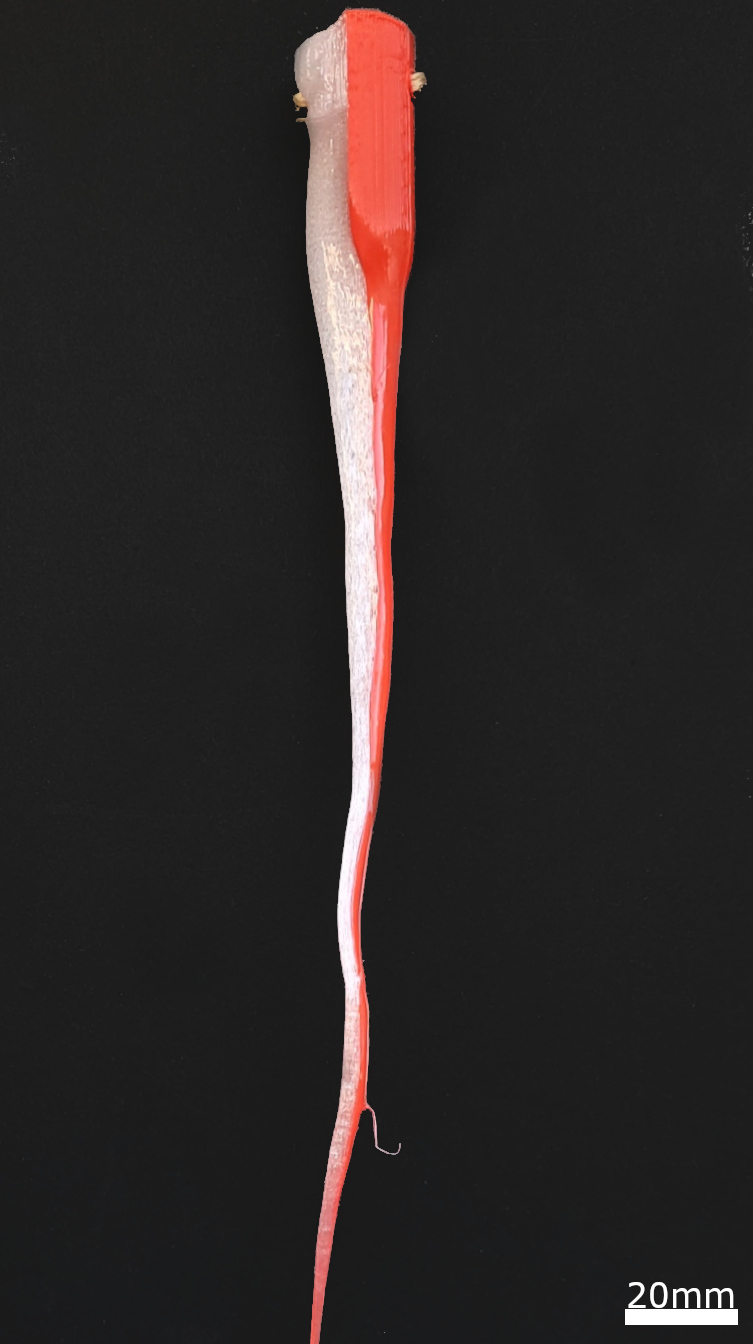
\includegraphics[width=\textwidth]{Abbildungen/Versuche/probe4_w.jpg}
         \caption{\acs{petg}/\acs{pla} }
        \label{fig:probe4}
     \end{subfigure}
     \caption{Probenkörper aus verschiedenen Materialkombinationen}
      \label{fig:probenkoerper_vor}
        \end{figure}

 \begin{figure}[!h]
     \centering
     \begin{subfigure}[]{.29\textwidth}
         \centering
         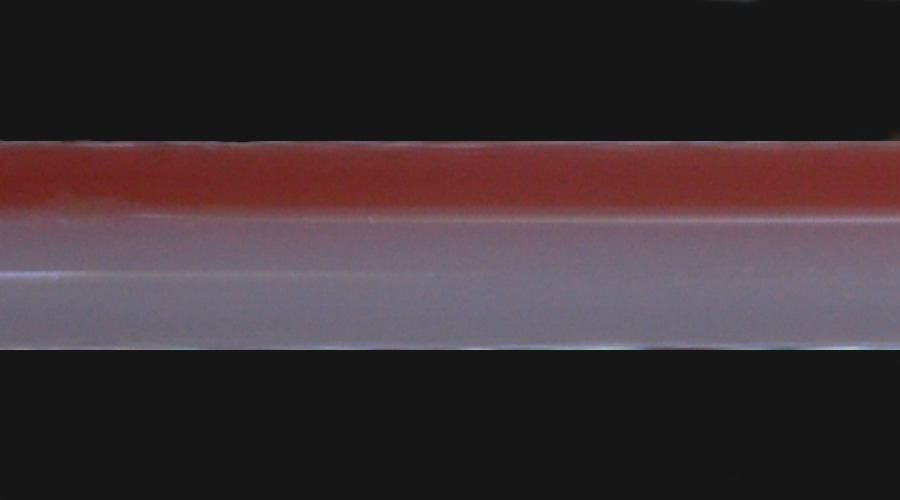
\includegraphics[width=\textwidth]{Abbildungen/Versuche/plapla_n.jpg}
         \caption{\acs{pla}/ \acs{pla}} 
         \label{fig:probe2_f}
     \end{subfigure}
     \hspace{5mm}
     \begin{subfigure}[]{.29\textwidth}
         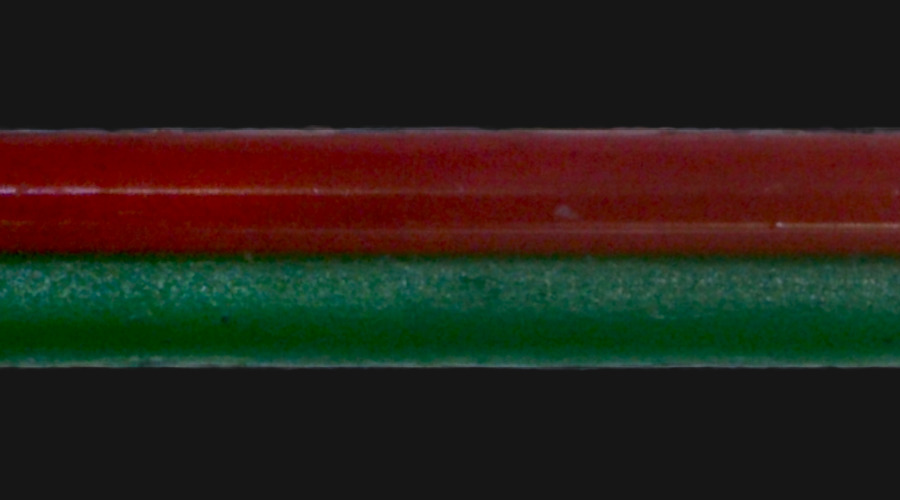
\includegraphics[width=\textwidth]{Abbildungen/Versuche/abspla_n.jpg}
         \caption{\acs{pla}/\acs{abs}}
         \label{fig:probe3_f}
     \end{subfigure}
     \hspace{5mm}
     \begin{subfigure}[]{.29\textwidth}
        \centering
        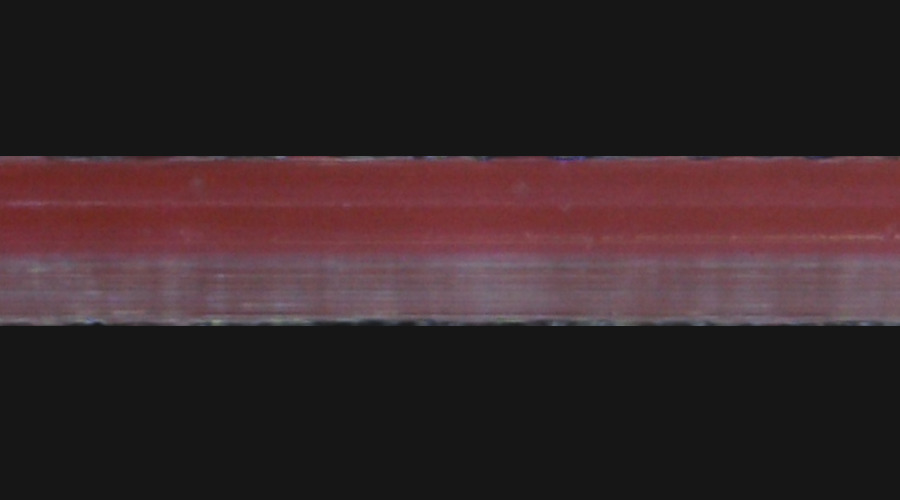
\includegraphics[width=\textwidth]{Abbildungen/Versuche/petgpla_n.jpg}
         \caption{\acs{petg}/\acs{pla} }
        \label{fig:probe4_f}
     \end{subfigure}
     \caption{Fasern aus verschiedenen Materialkombinationen}
      \label{fig:probenkoerper_vor}
        \end{figure}
    

Bei dem aktuell gewählten Prozess ist die Voraussetzung das sich beide Materialien des Probenkörpers, durch  erwärmen in ihrer Viskosität soweit herab gesenkt werden können das es ohne weiteren Eingriff in den Vorgang zu einer Ausbildung der Faser kommt. In der Zweiten Versuchsreihe sichtbar das dies zu problemen führen kann. In der Abbildung \ref{fig:probe2} wird ein Probenkörper aus zwei verschiedenen Farben \acs{pla} verwendet, was zum Ziel hatte das Erste Ergebnis zu replizieren und die Verteilung der Materialien zu beurteilen. Die Temperatur bei welcher sich der Prozess eingestellt hat liegt bei ca. 353°C. Dabei ist zu beachten das es sich bei der Angabe nicht um die Tatsächliche Materialtemperatur sondern um den Einstellwert des Rohrofens handelt. Die Materialtemperatur wurde nicht ermittelt, was jedoch während der Inbetriebnahme des gesamten Versuchsstandes und zur Stabilisierung des Prozesses in Betracht zu ziehen ist. Bei dieser Probe ist zu sehen das sich ein gleichmäßiger Abschmelzkegel (Abbildung \ref{fig:probe2}) sowie eine gleichmäßige Verteilung der \acs{pla}-Anteile (Abbildung \ref{fig:probe2_f}) ausbildet. Die ermittelte mittlere Faserdicke (Tabelle \ref{tab:erm_faserdicke}) ist ebenfalls inerhalb der Vorgaben. Anders als In Kapitel \ref{sec:therm} ist Sind die Probenkörper aus mehreren Materialien nicht mit einem stabil viskosem Mantel überzogen. So kann berurteilt werden ob dieser nötig ist oder ob es genügt wenn die Verarbeitungstemperaturen der Materialien eng beeinader liegen. In Abbildung \ref{fig:probe3} und \ref{fig:probe4} ist zu erkennen das der Abschmelzkegel sehr ungleichmäßig ist. Die Verabeitungstemperaturen von \acs{pla} und \acs{abs} liegen circa 30°C auseinader. Bei \acs{petg} und \acs{pla} sind es circa 40°C. Daraus lässt sich schließen das die Ausbildung eines gleichmäßigen Kegels maßgeblich von der Temperaturschere zwischen den gewählten Materialien abhängt. Das selbe Phänomen lässt sich auch bei der fertigen Faser erkennen. In Abbildung \ref{fig:probe3_f} ist zu sehen das die Verteilung der zwei Werkstoffe noch recht gleichmäßig ist, jedoch sind die zwei Halbzylinder nicht mehr vollständig an den Schnittfläche laminiert, was zu einer Sicke entlang der Grenzfläche führt. In Abbildung \ref{fig:probe4_f} ist die Temperaturdifferenz noch größer und so zeigt sich auch ein noch schlechteres Ergebnis. Zu sehen ist nur ein Dicke Schicht aus \ac{pla} mit einer ganz dünnen Anhaftung von \acs{petg}. Auch wenn die erreichten Dicken (Tabelle \ref{tab:erm_faserdicke}) innerhalb der Grenzwerte liegen ist das Ergebnis nicht Erwartungsgemäß. Da sich der Aufbau der Faser in den letzten zwei Versuchen nicht kontrollieren ließ ist es schwierig ein konstantes Ergebnis erzeugen, welches Später als Sensor oder Aktor verwendet werden kann.

\begin{center}
    \begin{table}[!h]
    \centering
        \begin{tabular}{c|c|c|c|c}
                Materialkombination & mittlere Dichte $\rho$ & Länge L & Masse m & Durchmesser d \\
                \hline
                \acs{pla}/\acs{pla} & $1,240 \frac{g}{cm^3}$ & $126 cm$ & $0,158g$ & $358\mu m$ \\
                \acs{pla}/\acs{abs} & $1,145 \frac{g}{cm^3}$ & $140 cm$ & $0,125g$ & $315\mu m$ \\
                \acs{petg}/\acs{abs} & $1,310 \frac{g}{cm^3}$ & $168 cm$ & $0,120g$ & $263\mu m$ \\
                
        \end{tabular}
        \\
        \begin{center}
            \begin{equation*}
                d = 2 \cdot \sqrt{\frac{m}{\rho * \pi * L}}
            \end{equation*}
        \end{center}
    \caption{Ermittelte Faserdicke}
    \label{tab:erm_faserdicke}
    \end{table}
\end{center}

Ein weiterer unbekannter Faktor ist die benötigte Abzugsgeschwindigkeit. Im Zuge einer Videoauswertung eines der Abzugsvorgänge konnte ein grober Richtwert von $72\frac{mm}{s}$ ermittelt werden.
Da es in dieser Studienarbeit mehr um die Entwicklung des Verfahrens und weniger um die Optimierung der Probenkörper geht sind die Erlangten Erkenntnisse sehr Hilfreich und bestätigen die Funktionsweise des Verfahrens grundsätzlich.


\newpage
\section{Abschätzung der Systemgeschwindigkeiten}\label{ch:systemspeed}

Da  der Rohrofen bereits vorliegt und nicht ausgesucht werden muss, stellt sich eher die Farge wie sich das Material im Temperaturfeld verhält und wie sich das auf die Faserdicke auswirkt. Das Vorliegende

\begin{wrapfigure}{l}{0.5\textwidth}
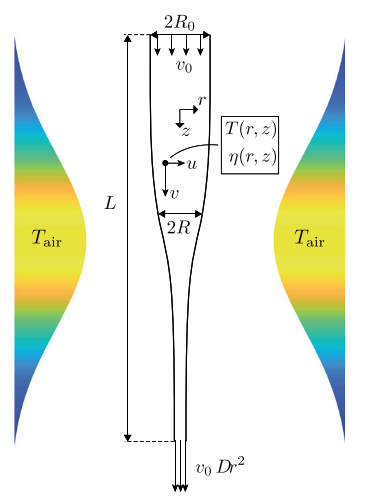
\includegraphics[width=0.9\linewidth]{Abbildungen/temp_field_clear.png} 
\caption{Temperaturfeld im Rohrofen
\cite{Page.2019} \vspace{1mm}}
\label{fig:thermal_field}
\end{wrapfigure}
 Berechnungsmodell bezieht sich ausschließlich auf Systeme welche vom verhalten durch ihr Mantelmaterial bestimmt sind. Es beschreibt das System im 2-Dimensionalen Raum, durch die Ausdehnenung $R(z)$ entlang der Hauptachse sowie durch ein Beschleunigungsfeld $u(r,z)$ in radialer- und $v(r,z)$ in axialer Richtung. Weiternen Einfluss nehmen das Temperaturfeld $T(r,z)$ sowie die Scherviskosität $\eta(r,z)$\cite{Page.2019}. Vorraussetzung für die Anwendbarkeit ist das vorhandensein einer dünnen Faser.
 \begin{equation}
     \alpha^2 = (\frac{R_0}{L})^2 \ll 1 \hspace{5mm}\cite{Page.2019} Gl.(1)
     \label{eq:fiber_thick}
 \end{equation}
Für den Fall des vorhandenen Ofens ergibts sich miitels Gleichung \ref{eq:fiber_thick} 
\begin{equation*}
    (\frac{R_{0max}}{L})^2 = (\frac{45mm}{500mm})^2 =8,1*10^{-3}
\end{equation*}
ein Wert der deutlich unter eins liegt und die Bedingung somit erfüllt.

\vspace{20mm}
 
Die größte unbekannte Unbekannte im Entwicklungsprozess ist das Fließverhalten des Halbzeugs. Da die bimorphe Faser aus mehren Materialien mit verschiedenen thermodynamischen Eigenschaften besteht, ist das Verhalten bei der Erwärmung schwer abzuschätzen. Da zum Zeitpunkt der Auslegung die Materialkombination nicht vorliegt, wird mit einer groben Näherung über die Kontinuitätsgleichung (Gl. (\ref{eq:kntinuitätsgleichubng})) gearbeitet.
\begin{equation}\label{eq:kntinuitätsgleichubng}
    v_1*A_1 = v_2*A_2
\end{equation}
Da die möglichen Durchmesser des Halbzeuga ($d_1 = [10, 45]mm$) sowie die  der  Faser ($ d_2 = [50*10^{-3}, 2]mm$) aus den Anforderungen hervorgehen, kann mit den Messwerten aus den Vorversuchen eine Abschätzung des Verhaltens getroffen werden.
\begin{equation}\label{eq:speed_v2}
    v_1 = v_2 * \frac{d_2^2}{d_1^2}
\end{equation}
Für die gemessene Materialkombination \acs{pla}/\acs{pla} ergibt sich mittels Gleichung \ref{eq:speed_v2} die folgende Fördergeschwindigkeit.
\begin{equation*}
    v_1 = 72\frac{mm}{s}*\frac{(358 * 1^{-3}mm)^2}{(18,5mm)^2} \approx 26,96 \frac{\mu m}{s}
\end{equation*}
Da davon Auszugehen ist das sich nicht alle Materialien gleich verhalten oder sich die Form der Probenkörper ändert wird der benötigte Geschwindigkeitsbereich um die Werte aus dem Versuch hervorgegangenen sind approximiert. 

\begin{figure}[!h]
     \centering
     \begin{subfigure}[]{0.4\textwidth}
         \centering
         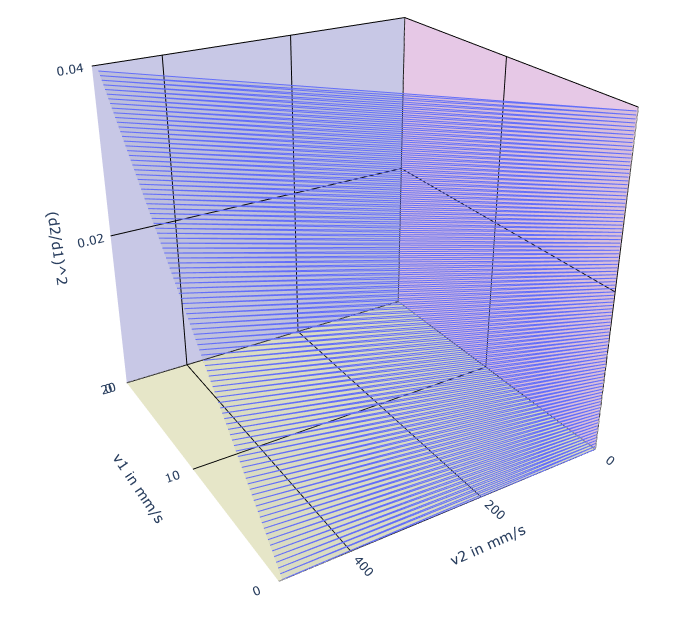
\includegraphics[width=\textwidth]{Abbildungen/v1_v2_d_wirframe_2 (2).png}
         
         \label{fig:abzug_speed}
     \end{subfigure}
     \hspace{0mm}
     \begin{subfigure}[]{0.2\textwidth}
         \begin{align*}
             v_{1min} = &  \ 1 \frac{mm}{s} * (\frac{200*10^{-3}mm}{45mm})^2 \approx 0,0198 \frac{\mu m}{s}\\      
             v_{1max} = &  \ 500  \frac{mm}{s} * (\frac{2mm}{10mm})^2 \approx 20 \frac{mm}{s}
         \end{align*}
         
         \label{fig:abzug_min_max}
     \end{subfigure}
     \caption{Abzugsgeschwindigkeiten}
      \label{fig:abzugsgeschwindigkeit}
\end{figure}

Die Entscheidung 500 $\frac{mm}{s}$ (Abbildung \ref{fig:abzugsgeschwindigkeit}) als maximale Abzugsgeschwindigkeit anzunehmen ist daraus begründet, das die im Versuch entstandene Faser bereits sehr nah an der unteren Dickengrenze liegt und das die Viskosität des Materials im Versuch sehr niedrig war. Deshalb gehe ich davon aus das ein Sicherheitsfaktor von circa 7 in der Abzugsgeschwindigkeit für viele mögliche Materialkombinationen ausreichend ist. 
So ergeben sich am ende zwei Geschwindigkeitsbereiche, einer für den Abzug und einer für die Materialfördereinheit. Dabei sit $v_1$ die Zuführgeschwindigkeit und $v_2$ die Abzugsgeschwindigkeit.
\begin{equation*}
    v_1 = [0,198\frac{\mu m}{s}; 20 \frac{mm}{s}] \hspace{20mm} v_2 = [1\frac{mm}{s};500\frac{mm}{s}]
\end{equation*}
         

 \newpage

\section{Abzug}
Der Abzug soll das Material aus dem Rohrofen abführen und die Faser in geeigneter Art und Weise für die Weiterverarbeitung auswerfen.
 \vspace{2mm}
\begin{enumerate}
    \item[]Die folgenden Bedingungen aus der Anforderungsliste sind zu erfüllen: \vspace{2mm}
    \item Die Dicke der abzuziehenden Faser soll je nach Material zwischen $200\mu m$ und  $ 2mm$ einstellbar sein (Tabelle \ref{tab:anforderungsliste} Punkt 5.1). Dabei ist zu beachten das aufgrund verschiedener Fließeigenschaften der Kunststoffe nicht alle Dicken des Bereichs erreichbar sind.
    \item Zur einfachen Weiterverarbeitung soll die Faser auf eine wechselbare Standardisierte Spule aufgewickelt werden (Tabelle \ref{tab:anforderungsliste} Punkt 5.2), welche sich einfach austauschen lässt (Tabelle \ref{tab:anforderungsliste} Punkt 5.3).
\end{enumerate}



\subsection{Varianten}
\begin{enumerate}[label=(\alph*)]

   \item \textbf{Aufrollen auf eine Spule} \label{Aufrollen_auf_eine Spule}\\
    Die abtropfende Faser wird unterhalb des Rohrs aufgefangen und direkt auf eine Spule aufgewickelt (Abbildung: \ref{fig:aufrollen}). Zur Einhaltung der angeforderten Standartspule wird für diese ein Außendurchmesser von $100mm$ angenommen. Die benötigte Motordrehzahl ist direkt vom Spulendurchmesser (Gl. (\ref{eq:drehzahlband_1})) abhängig.
    \begin{equation}\label{eq:drehzahlband_1}
        n = \frac{v}{ \pi * d} \hspace{3mm}\hspace{3mm} 
    \end{equation}
    Somit ergibt sich mittels Gleichung \ref{eq:drehzahlband_1}  das  benötigte Drehzahlband.
    \begin{equation*}
        n = [0,191;95,453]\frac{1}{min} 
    \end{equation*}
  
    Da die Drehzahlen sehr gering sind und davon ausgehen ist das es die benötigte Abzugskraft ebenfalls ist,ist ein Direktantrieb der Spule denkbar. In diesem Fall ist das aus der Beschleunigung der Spule hervorgehende Drehmoment das welches überwiegt. Diese Variante bringt aber auch einige Probleme mit sich. Zunächst ist die Steuerung der Abzugsgeschwindigkeit nicht ganz trivial. Die Antriebsgeschwindigkeit muss aufgrund des steigendes Spulendurchmessers während des Wickelns im laufe des Prozesses reduziert werden. Problematisch dabei ist den Aktuellen Spulendurchmesser zu bestimmen da dieser sowohl von dem Durchmesser der Faser als auch von  seiner Verteilung auf der Spule abhängt. Eine Weitere Herrausforderung ist der Start des Prozesses. So muss zu beginn die Faser auf die Spule aufgebracht werden um überhaupt einen Zug auf die Faser ausüben zu können. Alles in allem bedeutet die das Voraussetzung für für eine gute Regelbarkeit dieser Variante ist, das es eine Möglichkeit gibt die Faser initial in die Spule einzuhängen und das diese dann gleichmäßig über die Länge  verteilt wird.  
   
 
    \item \textbf{Abtriebsrollen} \label{abtriebsrollen_c}\\
    Die Faser wird unterhalb des Heizrohrs zwischen zwei relativ kleine Rollen geklemmt, welche sie vom Halbzeug abziehen (Abbildung: \ref{fig:abtreiben}). Die Berechnung erfolgt anlago zu \ref{Aufrollen_auf_eine Spule}. Nur der Spulendurchmesser ist nun der Rollendurchmesser, welcher auf $10mm$ festgelegt wird. Das Drehzahlaband für den Motor, in diesem Fall, ergibt sich somit wie folgt.
    \begin{equation*}
        n = [1,910;954,9230]\frac{1}{min}
    \end{equation*}
    Zu erkennen ist direkt das die Benötigten Drehzahlen um den Faktor 10 größer sind, da die Werte jedoch nicht zu groß sind ist dies zunächst kein Punkt, der der Variante negativ ausgelegt werden kann. Anzumerken ist aber das die Rollen die Faser mit geeigneter Kraft klemmen müssen damit gezogen werden kann. Dabei darf die Anpresskraft jedoch nicht so groß sein das es zu einer Beschädigung der Faser kommt. Da Verschiedenen Materialeien mit diversen Festigkeiten verwedet werden könnten ist die Kraft dem aktuellen Bedingungen immer anzupassen. Die Ermittlung der jeweils benötigten kraft ist Vermutlich nur durch Versuche möglich, da die Faser aus mehreren Materialien besteht und sich ja nach Rotation um ihre Längsachse  unterschiedlich verhalten kann. Zudem sollten beide Räder Angetrieben sein um die Reibung auf der Faser zu minimieren. 
    

     \begin{figure}[!h]
     \centering
     \begin{subfigure}[]{5cm}
         \centering
         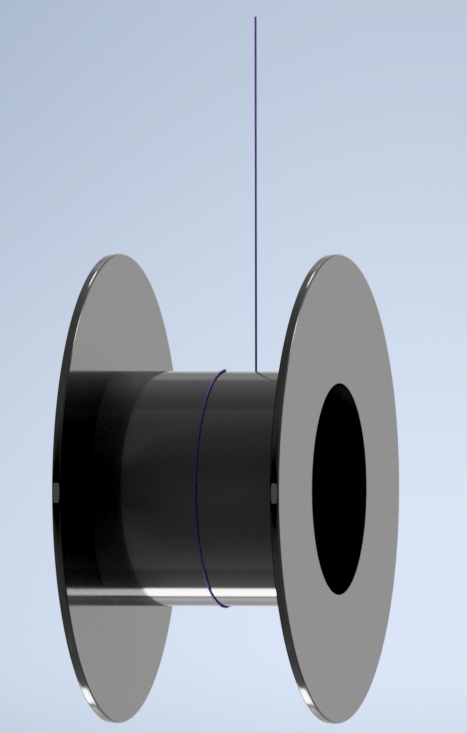
\includegraphics[width=\textwidth]{Abbildungen/aufrollen.png}
         \caption{}
         \label{fig:aufrollen}
     \end{subfigure}
     \hspace{10mm}
     \begin{subfigure}[]{5.4cm}
         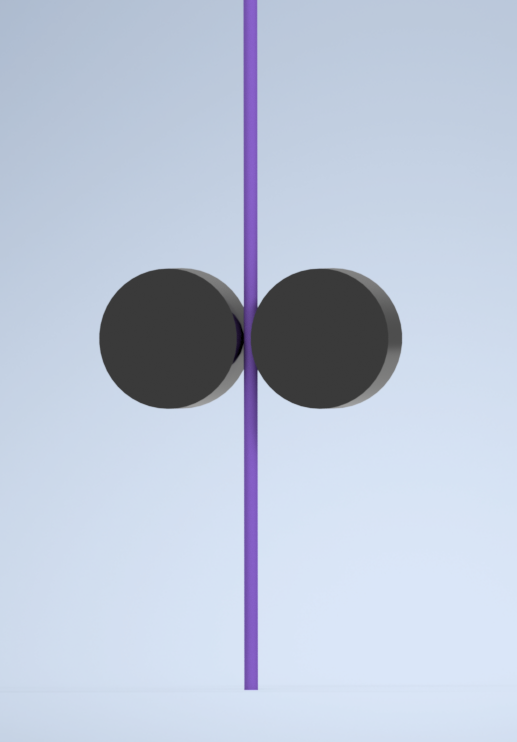
\includegraphics[width=\textwidth]{Abbildungen/abtriebsrollen.png}
         \caption{}
         \label{fig:abtreiben}
     \end{subfigure}
     \caption{Abzugsvarianten}
      \label{fig:abzugsvarianten}
        \end{figure}
        
   

    \item \textbf{Auswahl}\\
    Beide Varianten haben in gewissen Bereichen Vorteile und in anderen Nachteile. Jedoch gibt es bei Variante \ref{abtriebsrollen_c} den entscheidenden Nachteil das nach dem Abtreiben die Faser nirgends aufgenommen wird. Das führt dazu, das mit einer zusätzlichen Baugruppe, eine Lösung geschaffen werden muss. Da die naheliegende Möglichkeit der Aufnahme, der Faser, das Aufrollen ist, wären bei diesem Ansatz die Komponenten von Variante \ref{Aufrollen_auf_eine Spule} zusätzlich vonnöten. Aus diesem Grund werden die Nachteile von Variante \ref{Aufrollen_auf_eine Spule} in kauf genommen. Da diese Art der Konstruktion ebenfalls simpler und mit einem niedrigeren Drehzahlband einhergeht ist sie für einen Prototypen am geeignetsten. Sollte sich während der Konstruktion und Erprobung herausstellen das die Geschwindigkeitssteurung in diesem Fall zu instabil ist, können die Abtriebsrollen nachgerüstet werden.
    
\end{enumerate}
\newpage

\subsection{Dimensionierung und Komponentenauswahl}

%\begin{enumerate}[label=(\alph*)]

\subsubsection{Antriebsmoment an der Spule}
Die zum abziehen der Faser benötigten Kräfte sind sehr klein und werden deshalb im nachfolgenden vernachlässigt. Somit ist das aufzubringende Antriebsmoment ausschließlich von der Massenträgheit und der Beschleunigung abhängig. Um die Berechnung zu vereinfachen wird eine konstante Beschleunigung angenommen. \\
\textit{Weiterhin werden folgende Annahmen getroffen:}
\begin{center}
    \begin{table}[!h]
        \begin{tabular}{ll|ll}
             Maximaldrehzahl & $n_{max}=95,453min^{-1}$ &
             Spulenhöhe & $h=0,07m$ \\
             Spuleninnendurchmesser & $d_i = 0,1m$ &
             Spulenaußendurchmesser & $d_a = 0,2m$\\
             maximale Materialdichte & $\rho = 3000 \frac{kg}{m^3}$ &
             Beschleunigungszeit & $t_0 = 4s$   
        \end{tabular}
    \caption{Kennwerte zur Berechnung des Antriebsmomentes}
    \label{tab:geg_antriebsmoment}
    \end{table}
\end{center}
Die Gleichung \ref{eq:antriebsmoment_aus_trägheit} kann nun zur berechnung verwendet werden. 
\begin{equation}\label{eq:antriebsmoment_aus_trägheit}
     M =  J_P \cdot \Ddot{\varphi}
\end{equation}

Um die Massenträgehit $J_P$ zu berechnen wird in erster Linie nicht die Masse der Spule benötigt. Es ist zwar in der Regel davon auszugehen das die Spule nur leer, zu beginn des Prozesses, beschleunigt werden muss jedoch wird aus Gründen der Flexibilität die Anlage so ausgelegt das die Beschleunigung auch mit voller Spule möglich ist. 
\begin{equation}\label{eq:masse_von_d}
    m = (d_a^2-d_i^2) \cdot \frac{\pi \cdot h \cdot \rho}{4}
\end{equation}
Vereinfacht betrachtet ist die Spule ein Hohlzylinder weshalb die Masse mit Gleichung \ref{eq:masse_von_d} berechnet werden kann. Der äußere Durchmesseer $d_a$ steigt dabei je mehr Faser aufgewickelt wurde. Um auch hier einfach zu bleiben werden die beim aufwickeln entstehenden Freiräume nicht berücksichtigt. 
\begin{equation}\label{eq:polare_Jp}
    J_P = m \cdot \frac{d_a^2+d_i^2}{8}
\end{equation}
So kann mit  Gleichung \ref{eq:polare_Jp} und \ref{eq:masse_von_d} das Polare Massenträgheitsmoment der Spule vollständig beschrieben werden.
\begin{equation}
    J_P = \frac{\pi \cdot h \cdot \rho}{32} \cdot (d_a^4-d_i^4)
\end{equation}

Nun wird noch die Winkelbeschleunigung benötigt, welche sich aus der ersten Ableitung der Winkelgeschwindigkeit ergibt.
\begin{equation}\label{eq:winkelgeschwinigkeit}
    \dot{\varphi} = 2\pi n
\end{equation}
Da die Drehzahl Zeitveränderlich ist kann sie mit den angaben aus Tabelle \ref{tab:geg_antriebsmoment} wie folgt beschrieben werden.
\begin{equation}
    n= \frac{n_{max}}{t_0} \cdot t
\end{equation}
Somit folgt die Winkelbeschleunigung.
\begin{equation}\label{eq:winkelbneschleunigung}
    \Ddot{\varphi} = 2\pi \frac{n_{max}}{t_0}
\end{equation}
Werden jetzt alles Teile zusammengesetzt entsteht die Gleichung \ref{eq:m_from_J}, welche eine Aussage über das benötigte Moment zum beschleunigen der Spule in Abhängigkeit vom Füllstand trifft.
\begin{equation}\label{eq:m_from_J}
    M = \frac{\pi ^2 \cdot n_{max} \cdot h \cdot \rho}{16 \cdot t_0}\cdot(d_a^4-d_i^4)
\end{equation}
Da vorher festgelegt wurde das die Momente nach dem Beschleunigen zu vernachlässigen sind, entspricht das Beschleunigungsmoment $M$ dem benötigten Antriebsmoment $M_G$.

\begin{figure}[!h]
    \centering
    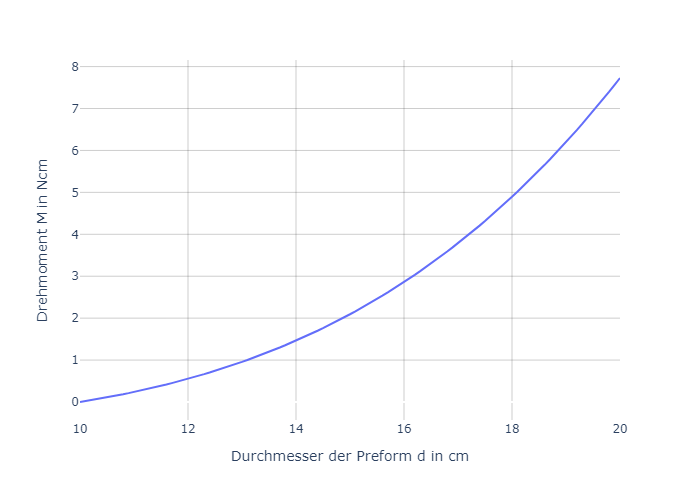
\includegraphics[width = 0.6\textwidth]{Abbildungen/MG_from J.png}
    \caption{Benötigtes Antriebsmoment bei verschieden Füllständen der Spule}
    \label{fig:MG_fromJP}
\end{figure}

Die Abbildung \ref{fig:MG_fromJP} Zeigt den Drehmomentsanstieg für die Beschleunigung bei unterschiedlichen Füllständen der Spule. Das größte Moment was daraus hervorgeht beträgt circa $7,5 Ncm$. Lässt sich für das Drehzahlband kein passender Motor finden ist auch der Einsatz eines Getriebes möglich. Damit der Aufbau möglichst einfach bleibt könnte ein Synchrongetriebe verwendet werde. Diese haben einen hohen Wirkungsgrad und die Übersetzung lässt sich leicht anpassen.
\begin{equation}\label{eq:uebersetzung}
     i=\frac{z_2}{z_1} = \frac{n_1}{n_2} \hspace{10mm} \cite{DIN77212.Juni1989}
\end{equation}

Mit Gleichung \ref{eq:uebersetzung} lässt sich mit der Drehzahl des Motors die Passende Übersetzung berechnen. Synchrongetriebe besitzen einen Wirkungsgrad ($\eta$) der größer als $0,98$ ist \cite{DIN77212.Juni1989}.
\begin{equation}\label{eq:m_synchrongetriebe}
    M_G = M*\frac{z_2}{z_1}\frac{1}{\eta} \hspace{10mm} \cite{DIN77212.Juni1989}
\end{equation}

Das Angepasste Antriebsmoment ($M_G$) ist also von der Zähnezahl der Riemenscheiben abhängig die so berechnet werden müssen das Drehmoment und Drehzahl zu Forderung passen.

%-----vlllt b ab hier ---- auswahl motor%


\subsubsection{Spulenaufnahme}
Die Aufnahme der Spule muss sicherstellen das Sie nicht Durchrutschen kann, da darüber die Kraft auf die Faser wirkt. Da die Spule mit einer Zentralschraube befestigt wird (Abbildung \ref{fig:halbschnitt_Spule}), muss diese das Antriebsmoment aufnehmen können.

\begin{figure}[!h]
    \centering
    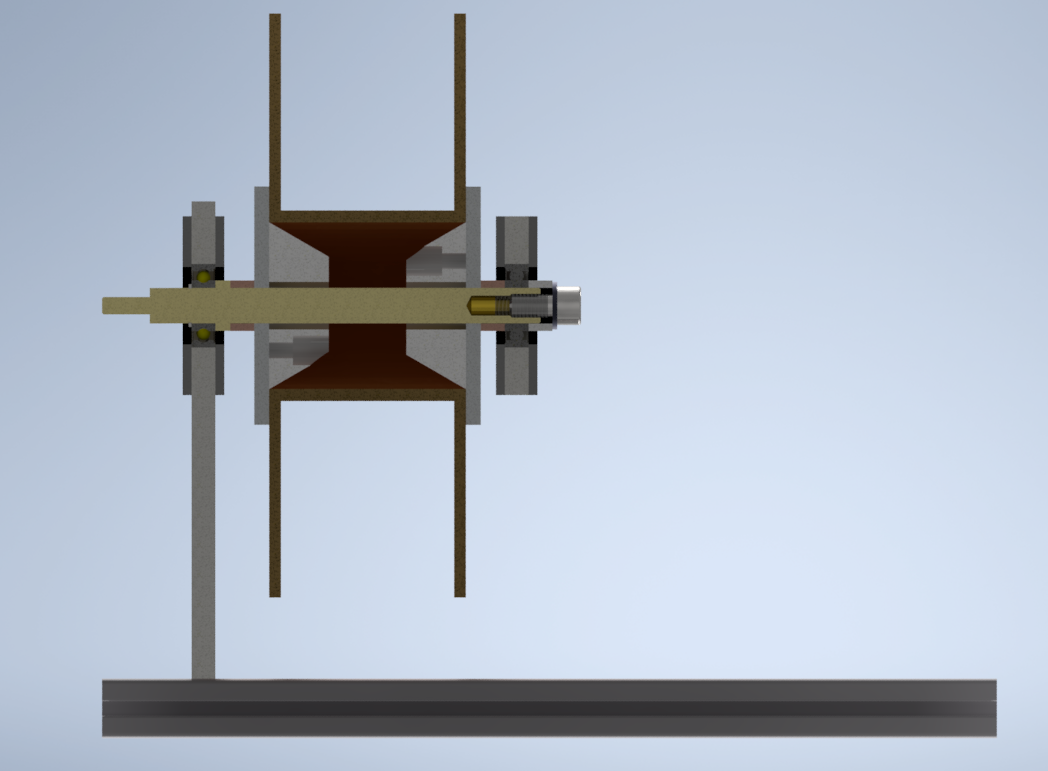
\includegraphics[width = 0.7\textwidth]{Abbildungen/Spulenaufnahme_0.png}
    \caption{Hablschnitt des Abzugs}
    \label{fig:halbschnitt_Spule}
\end{figure}

Um dies Sicherzustellen wird das benötigte Anzugsmoment der Schraube berechnet.
\begin{equation}\label{eq_MA_DIN}
    M_A = F_{Mmax}\cdot(0,16 \cdot P + 0,58\cdot d_2 \cdot \mu_{Gmin} + \frac{D_{KM}}{2}\cdot \mu_{Kmin}) \hspace{10mm} \cite{VDI2230Blatt1.November2015}
\end{equation}

Dabei ist $F_{Mmax}$ die Vorspannkraft der Schraube, welche zum übertragen des Antriebsmomentes benötigt wird. 
\begin{equation}\label{eq_Fmmax}
     F_{Mmax} = \frac{M_{Motor}}{r_a \cdot \mu_{Tmin}} \hspace{10mm} \cite{VDI2230Blatt1.November2015}
\end{equation}
Zur Berechnung wird nun das maximale Drehmoment des Motors ($M_{Motor} = 3Nm$) verwendet, auch wenn dieses viel größer ist als das benötigte Antriebsmoment. Sollte der Motor aus irgendeinem Grund, während des Prozesses, dieses Drehmoment Aufbringen soll sich die Schraubverbindung trotzdem nicht lösen. Unter Verwendung der Haftreibung zwischen Stahl und Stahl ($\mu_{Tmin}$) von circa $0,15$ und dem effektiven Radius ($r_a = 5,25mm$) des Schraubenkopfes der M8 schraube lässt sich die Vorspannkraft und somit auch das Anzugsmoment berechnen. Die Gewindesteigung $P$ beträgt $1,25mm$, der Flankendurchmesser $d_2$ der Schraube beträgt $7,188mm$ und der Wirksame Kopfdurchmesser $D_{KM}$ ist $10,5mm$. Benötigt werden nun nur noch die Haftreibzahl der Kopfauflage ($\mu_{Kmin}$) von $0,15$ und die Haftreibung im Gewinde ($\mu_{Gmin}$) mit einen Wert von $0,12$.
\begin{equation}\label{eq:solve_MA}
        M_A \approx 5,668 Nm
\end{equation}
Da eine M8 8.8 Schraube mit bis zu $24Nm$ belastet werden darf kann die Spule so befestigt werden.




\section{Materialzufuhr}
Die Materialzufuhr besteht aus mehreren Problemstellungen. Es muss ein Probenkörper Senkrecht über dem Heizrohr befästigt werden, welcher dann vertikal verfahren werden kann.



\begin{enumerate}
    \item[]Die folgenden Bedingungen aus der Anforderungsliste sind zu erfüllen: \vspace{2mm}
    \item Die maximal zu förderende Länge eines Probenkörpers soll $500mm$ betragen (\ref{tab:anforderungsliste} Punkt 6.1)
    \item Es sollen Proformen mit Durchmessern von $10mm-45mm$ verwendbar sein (\ref{tab:anforderungsliste} Punkt 6.2).
    \item Außerdem sollen verschiedene Querschitte ( Rund, Quader) von Probenkörpern aufgenommen werden können.
\end{enumerate}

\subsection{Varianten}
Zur besseren Differenzierbarkeit werden verschiedene Varianten für die Linearführung und für die Aufnahme des Probenkörpers  diskutiert.

\subsubsection{Linearführung}
Zur Förderung von Material gibt es Prinzipiell zwei Varianten. Erstens die Probe kann mit einer Linearachse und eine entsprechenden Aktor bewegt werden. Zweitens, sie kann ,ähnlich wie bei der Faser, zwischen zwei getriebenen Rollen eingeklemmt und nach unten gefördert werden. 

\begin{enumerate}[label=(\alph*)]
    \item \textbf{Linearchse}\\
    In Abbildung \ref{fig:linearachse} ist der Aufbaue einer Linearchse dargestellt. Neben dieser Variante gäbe es noch die Möglichkeit die in der Mitte der Darstellung verwendete Trapezgewindespindel durch ein anderes System zu Ersetzen.Geeignet dafür wären sowohl Hydraulische als auch Pneumatische Zylinder. Zu beachten ist aber das der Kostenaufand für ein solchen Aktor viel größer sind. Weiterhin ist auch der Wartungsaufwand und die Fehleranfälligkeit viel größer. Das liegt zum einen daran das beide Alternativen niemals zu hundert Prozent dicht sind und es das es im Fehlerfall nicht nur zum Ausfall sondern auch zu Leckagen kommen kann, was im Falle eines Hydraulischen Systems einem großen Reperaturaufand bedeuten würde.
    \begin{figure}[!h]
        \centering
        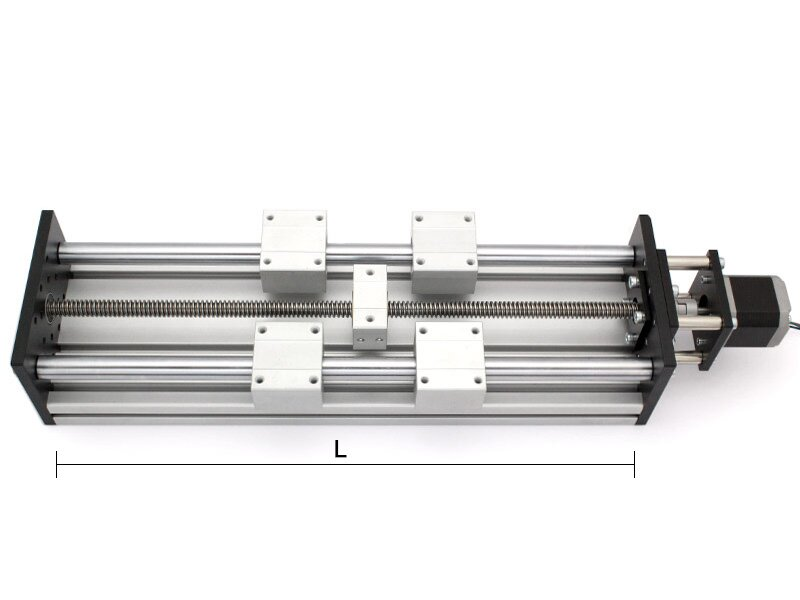
\includegraphics[width = 0.5\textwidth]{Abbildungen/linearachse-konfigurator-easy-mechatronics-system-1216a-nennlaenge-150mm~2.jpg}
        \caption{Beispiel einer Linearachse \cite{LinearachseDOLD.}}
        \label{fig:linearachse}
    \end{figure}
    
    Bei der Verwendung eines Motors in Kombination mit einer Spindel, wie in Abbildung \ref{fig:linearachse}, ist sowohl der Wartungs- als auch der Kostenaufand gering. Wenn bei diesem Aufbau der Motor ausfällt hat es keine weiteren Folgen und er kann einfach ersetzt werden. Zu diskutieren ist noch welche Art von Spindelgetriebe verwendet werden sollte. Es gibt die Variante mit Trapezgewindespindel und die mit Kugelumlaufspindel. Was den Wirkungsgrad angeht ist die Trapezgewindespindel unterlegen, da diese Gleitreibung im Gewinde besitzt. Die Kugelumlaufspindel sitzt nicht in einem klassischem Gewinde sondern wird mit wird durch eine Mutter geführt die Kugeln statt eines Gewindes besitzt. Das führt neben der geringeren Reibung auch zu einer längeren Standzeit. Nachteilig ist jedoch das sie keine Selbsthemmung besitzt und so die Achse im stromlosen Zustand nach unten fällt, da sie vertikal verbaut werden muss. Da die zuvor berechneten Kräfte und Geschwindigkeiten sehr klein sind ist der Wirkungsgrad nicht entscheidend. Der wesentliche Vorteil der Trapezgewindespindel ist der geringere preis weswegen diese für einen ersten Prototypen zu wählen ist.
    Diese Variante ist somit Preiswert und Flexibel, da auf die Achse alle möglichen arten von Materialhaltern montiert werden kann ohne die Steuerung oder das Getriebe verändern zu müssen.

    \item \textbf{Abtriebsrollen}\\
    Eine weitere möglichkeit ist ein ähnliches vorgehen wie Variante (b) bei dem Abzug. Dazu würde der Probenkörper zwischen zwei rollen geklemmt und nach unten gedrückt werden. In Abbildung \ref{fig:abtrieb_mat} ist eine Entwurf eines solchen Systems zu sehen. Es ist wichtig zu beachten das sich je nach Durchmesser des Probenkörpers die Auflagefläche in den Rollen ändert, was dazu führen kann das zu wenig Reibung vorherrscht. Deswegen wäre hier für jeden Durchmesser eine andere Aufnahme von Nöten. Dies gilt auch wenn an andere Querschnitte wie Quader gedacht wird. Vorteilhaft ist das diese Variante platzsparender ist und theoretisch beliebig lange Probenkörper zulässt.
  
    \begin{figure}[!h]
        \centering
        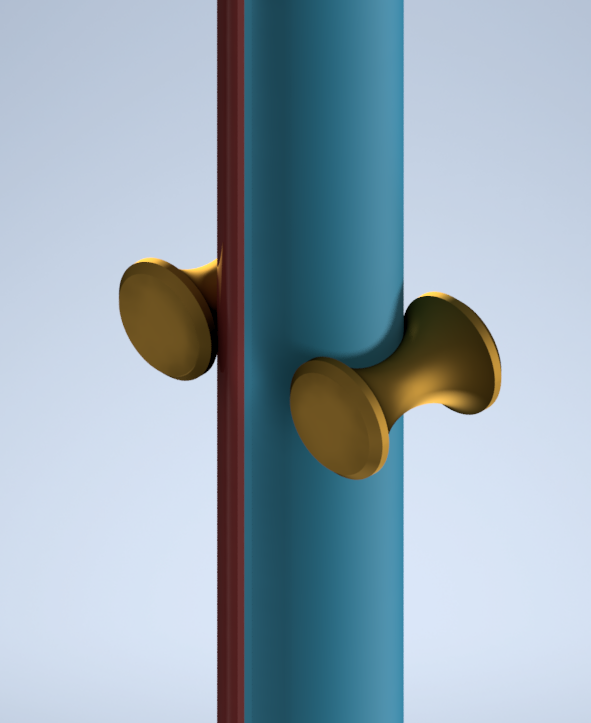
\includegraphics[width = 0.4\textwidth]{Abbildungen/abtrieb_mat.png}
        \caption{Abtriebsrollen für die Materialförderung}
        \label{fig:abtrieb_mat}
    \end{figure}
    
    \newpage
    
    \item \textbf{Auswahl}\\
    Da die Linearachse eine einfachere Modifizierbarkeit sowie besitzt und sie als fertiges Kaufteil erworben werden kann ist sie die bessere Wahl. Mit verschieden Anbauteilen lässt sich die Ache für ein breites Spektrum an Probenkörpern verwenden. 
    Das mit der Linearachse keine beliebig langen Teile verarbeitet werden können spielt bei ein Versuchstand keine Rolle da zunächst eher kleine Proben in verschieden Konfigurationen verwendet werden sollen. 



\end{enumerate}

\subsubsection{Materialhalterung}
Aus dem oberen Vergleich geht hervor das eine Linearchse verwendet wird, weshalb hier nur verschiedene Halterungen für diesen Typ Achse diskutirt werden.

\begin{enumerate}[label=(\alph*)]

\item \textbf{Spannfutter}\\
Eine möglichkeit der Befestigung ist die Verwendung eines Spannfutters, wie es auch bei einer Drehbank zum einsatz kommt. 

\begin{figure}[!h]
    \centering
    \includegraphics[width = 0.3\textwidth]{Abbildungen/Präzisions 4 Backenfutter.jpg}
    \caption{Spannfuter 160mm für Drehbänke \cite{MUK24.13.01.2024}}
    \label{fig:spannfutter}
\end{figure}

In Abblidung \ref{fig:spannfutter} ist ein solches zu sehen. Je nach Ausführung lassen sich die in der Mitte befindlich Backen auf ein variables Maß einstellen und können so verschiedenste Größen von Probenkörper aufnehmen. Werden nun noch ein paar Adapter (zum Beispiel eckig zu rund) beigelegt können auch variable Querschnitte aufgenommen werden. Ein weitere Vorteil ist das die Probe immer beim festziehen automatisch zentriert wird. Negativ zu Betrachten ist das diese futter sehr schwer sind, da sie im Originalen Einsatzfeld relativ große Kräfte aushalten müssen. Für den Versuchsstand sind sie demzufolge Überdimensioniert da die auftretenden Kräfte dort sehr klein sind.

\item \textbf{Klemmbacken}\\
Eine einfachere Variante ist der Einsatz von Klemmbacken, wie in Abbildung \ref{fig:klemm_linear}. Diese funktionieren im Prinzip wie eine Schraubzwinge. Mit einer Schraube wird eine der blauen Backen so weit in dieMitte gedreht das sich die Probe über der Mitte des Rohrofens befindet. Dann wird die zweite Seite dagegen geschoben und fixiert so die Probenkörper. Je nach dem wie viel Drehmoment auf die Vorrichtung gegeben wird können Preformen unterschiedlich stark geklemmt werden. 

\begin{figure}[!h]
    \centering
    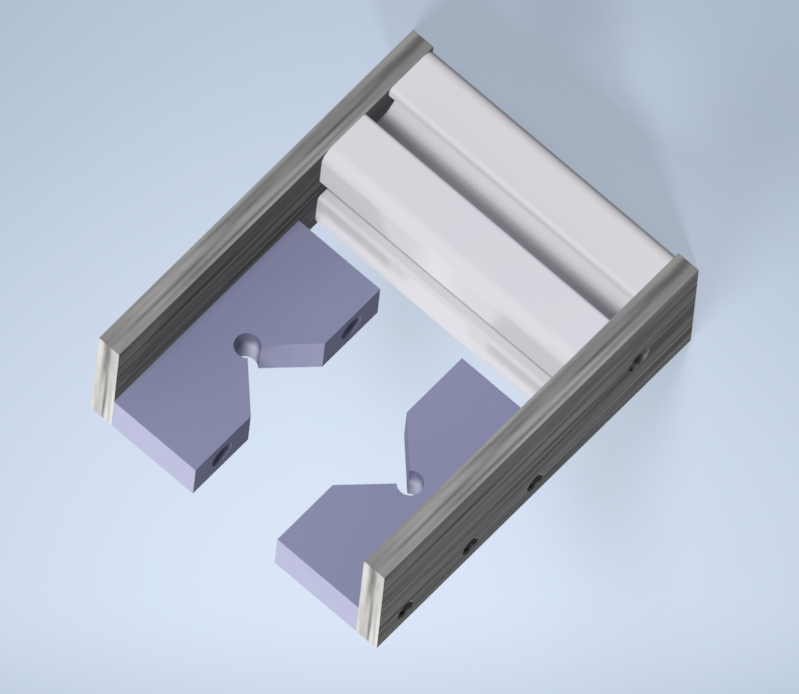
\includegraphics[width = 0.5\textwidth]{Abbildungen/aufnehmer_linear.png}
    \caption{Klemmbacken zur Halterung von Probenkörpern}
    \label{fig:klemm_linear}
\end{figure}

Diese Variante ermöglicht außerdem die Halterung von runden und eckigen Querschnitten ohne Umbau oder den Einsatz von Adaptern. Der Nachteil zu vorherigen Variante ist das der Probenkörper nicht automatisch zentriert wir, weshalb die Einrichtung einer Probe etwas schwieriger ist.

\item \textbf{Auswahl}\\
Die Erste Variante ist zwar klar die bessere, jedoch ist sie auch wesentlich teurer und schwerer. Damit der Versuchsstand so einfach und kosteneffizient wie möglich bleibt fällt die Wahl auf Variante (b), zum großen Teil auch deswegen weil sie viele verschiedene Probenkörper ermöglicht.

\end{enumerate}


\subsection{Dimensionierung und Komponentenauswahl}

\subsubsection{Linearführung}
Zur Linearführung sind alle wirkenden Lasten zu berechnen um sicherzustellen das die Trapezgewindespindel diesen Standhält. Ebenfalls muss ein Motor ausgelegt werden der die entsprechenden Lasten bewegen kann.

\begin{enumerate}[label=(\alph*)]
    \item \textbf{Axialkraft}\\
    Die einzige Last die auf das System wirkt ist jene, welche vom  Eigengewicht des Probenkörpers ausgeht.
    \begin{equation}\label{eq:mg}
        F = m\cdot g
    \end{equation}
    Die zu auf die Spindelmutter wirkende Axialkraft $F$ ergibt sich so mit Gleichung \ref{eq:mg}. Da die Masse noch Unbekannt ist muss diese Ermittelt werden. 
    \begin{equation}\label{eq:masse}
        m = \frac{\pi \cdot d^2}{4} \cdot L \cdot \rho
    \end{equation}
    Zur Abschätzung der maximalen Masse wird ein zylindrischer Probenkörper mit einem Durchmesser $d=50mm$ und einer Länge $L = 500mm$ angenommen. Die dichte der Probenkörper varriert je nach Materialkombination. Die mittlere Dichte der meisten verwendbaren Materialien liegt bei circa $1,5 \frac{g}{cm^3}$. Um auch Materialkombinationen abzudecken die nicht im Entwurf bedacht wurden wird mit einem Sicherheitsfaktor von zwei, eine maximale mittlere Dichte $\rho$ von $3,0\frac{g}{cm^3}$ angenommen.
    \begin{equation} \label{eq:F_final}
        F = \frac{\pi \cdot d^2}{4} \cdot L \cdot \rho \cdot g
    \end{equation}
    Mit Gleichung \ref{eq:F_final} und einer Fallbeschleunigung von $g =  9,81 \frac{m}{s^2}$ ergibt sich die auf die Trapezgewindemutter maximal wirkende Kraft (Gleichung \ref{eq:solve_F}).
    \begin{equation}\label{eq:solve_F}
        F = \frac{\pi \cdot (0,05m)^2}{4} \cdot 0,5m \cdot 3000\frac{kg}{m^3} \cdot 9,81\frac{m}{s^2} = 28,893N
    \end{equation}


    \item \textbf{Knickbeanspruchung}\\
    Da die Gesamte Kraft (Gleicung \ref{eq:solve_F} von der Spindel gehalten werden muss, ist sicherzustellen das diese nicht abknickt. Aus dem Datenblatt des Herstellers lässt sich so mit Gleichung \ref{eq:fcp} die maximal zulässige Kraft auf die Spindel bestimmen.
    \begin{equation}\label{eq:fcp}
        F_{cp}= \frac{21\cdot10^4\cdot D_3 \cdot \pi ^3 \cdot f}{64 \cdot L_{cp}^2} \hspace{20} \cite{DOLDMechatronikGmbH.}
    \end{equation}
    
    Im vorliegenden Fall ist jedoch der benötigte Kerndurchmesser $D_3$ die unbekannte, da die maximal wirkende Kraft zuvor bereits berechnet wurde. 
    \begin{equation}
        D_3 = \frac{F_{cp}\cdot 64 \cdot L_{cp}^2}{21\cdot 10^4 \cdot \pi^3 \cdot f}
    \end{equation}
    \begin{figure}[!h]
        \centering
        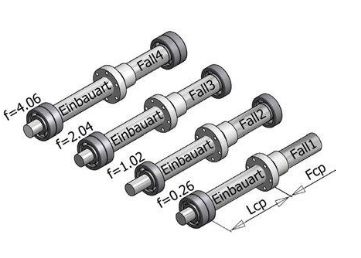
\includegraphics[width=0.5\textwidth]{Abbildungen/Lagerungstyp.png}
        \caption{Lagerungstypen für Spindeltriebe \cite{DOLDMechatronikGmbH.}}
        \label{fig:lagerung_knick}
    \end{figure}

    Angenommen wird eine Lagerung $f=1,02$ aus Abbildung \ref{fig:lagerung_knick}. Somit ergibt sich mit der Kraft aus Gleichung \ref{eq:solve_F} so wie einem maximalen Abstand zwischen Lager und Mutter von $L_{cp}~=~500mm$ der minimale Kerndurchmesser.
    \begin{equation}
        D_3 = \frac{28,893\cdot10^{-3}kN\cdot 64 \cdot (500mm)^2}{21\cdot 10^4 \cdot \pi^3 \cdot 1,02} \approx 6,93\cdot10^{-2} mm
    \end{equation}
    Da der die Kraft und dadurch der benötigte Kerndurchmesser sehr klein sind können praktisch alle Größen von Trapezgewindespindeln verwendet werden. Es wird im weiteren von einer Spindel mit einem Flankendurchmesser von $12mm$ ausgegangen.

    \item \textbf{Antriebs- und Haltemoment}\\
     Um die last bewegen zu können ist ein bestimmtes Drehmoment am Motor erforderlich. Da dieses sehr stark von der Steigung der Spindel abhängt wird die Berechnung für einen Festgelegten wert für die Steigung durchgeführt. Aus Kapitel \ref{ch:systemspeed} wissen wir das die benötigten Geschwindigkeiten sehr klein sind jedoch präzise gesteuert werden müssen. Aus diesem Grund wird die kleinste, beim gewählten Hersteller angebotene, Steigung $P$ von  $3mm$ verwendet. Da jede Art von Getriebe verlustbehaftet ist wird mit Gleichung \ref{eq:spinde_wiirkungsgrad} zunächst der Wirkungsgrad bestimmt.
     \begin{equation}\label{eq:spinde_wiirkungsgrad}
         \eta = \frac{tan(\alpha)}{tan(\alpha+\beta)} \hspace{10mm} \cite{DOLDMechatronikGmbH.}
     \end{equation}
     Um den Reibungswinkel $\beta$ und den Steigungswinkel $\alpha$ zu berechnen werden die Gleichungen \ref{eq:steig_w} und \ref{eq:reib_w} verwendet.
     \begin{align}
         &\alpha = arctan(\frac{P}{D_2\cdot \pi})  \hspace{10mm}\cite{DOLDMechatronikGmbH.}\label{eq:steig_w} \\
         &\beta = arctan(\mu G) \hspace{16mm}\cite{DOLDMechatronikGmbH.}\label{eq:reib_w}
     \end{align}
     So ergibt sich mit dem Flankendurchmesser $D_2$ von $12mm$ und einem Reibungskoeffizienten von $\mu G = 0,05$ \cite{DOLDMechatronikGmbH.} der Wirkungsgrad $\eta$ (Gleichung \ref{eq:eta}).
     \begin{equation}\label{eq:eta}
         \eta = \frac{P}{D_2\cdot \pi \cdot tan(arctan(\frac{P}{D_2  \pi})+arctan(0,005))} \approx 0,6117
     \end{equation}

     Das benötigte Antriebsmoment lässt nun für die Auslegung des Motors bestimmen.
     \begin{equation}\label{eq:FtoMa}
         M_A = \frac{F \cdot P}{2000 \cdot \pi \cdot \eta} \hspace{10} \cite{DOLDMechatronikGmbH.}
     \end{equation}

    Mit Gleichung \ref{eq:FtoMa} lässt sich das minimal nötige Drehmoment berechnen. Dazu wird für $F$ der wert aus Gleichung \ref{eq:solve_F} verwendet.
    \begin{equation}
        M_A = \frac{28,893N \cdot 3mm}{2000\pi \cdot 0,6117 } = 0,0225 Nm \approx 2,25 Ncm
    \end{equation}

    Da $\alpha$ im falle einer Geschmierten welle und einer Bronzemutter größer als $\beta$ ist, ist die Trapezgewindespindel nicht Selbsthemmend \cite{DOLDMechatronikGmbH.}. Das hat zur folge das der gewählte Motor ein neben dem berechneten Antriebsmoment auch ein ebenso großes Haltemoment vorweisen muss, damit bei perfekter Schmierung der Probenkörper im Stillstand an Ort und Stelle gehalten werden kann.
    
    \item \textbf{Komponentenauswahl}

    Da der Durchmesser der Trapezgewindespindel nicht von größere Bedeutung ist wird hier eine mit $12mm$ Flankendurchmesser und einer Steigung von $3mm$ gewählt. Anbieten würde sich für die ausgesuchte Führung ein Nema 17 bipolar-Steppermotor. Dieser hat ein Haltemoment von $51 Ncm$ und ein maximales Drehmoment von $35Ncm$ welches bei Steigerung der Drehzahl auf $1000min^{-1}$ auf circa $0,5Ncm$ sinkt (bei 24V). Damit entspricht er prinzipiell den Anforderungen. Zu Überprüfen ist nun nur noch ob die Maximaldrehzahl ausreichend ist.
    \begin{equation}
        v_1 = n_{max} \cdot P
    \end{equation}
    Damit kann der Motor eine Maximale Geschwindigkeit von $50 \frac{mm}{s}$ erreichen, was über der geforderten Geschwindigkeit von $20\frac{mm}{s}$ liegt.
    
    
    
     
    
\end{enumerate}


\subsubsection{Materialaufnahme ---Entfernen ---}




\section{Steuerung}
\subsection{Prozessbeschreibung - strukturierte Darstellung}
\subsection{Schaltungsentwurf}
\subsection{Implementierung}
